97. \begin{figure}[ht!]
\center{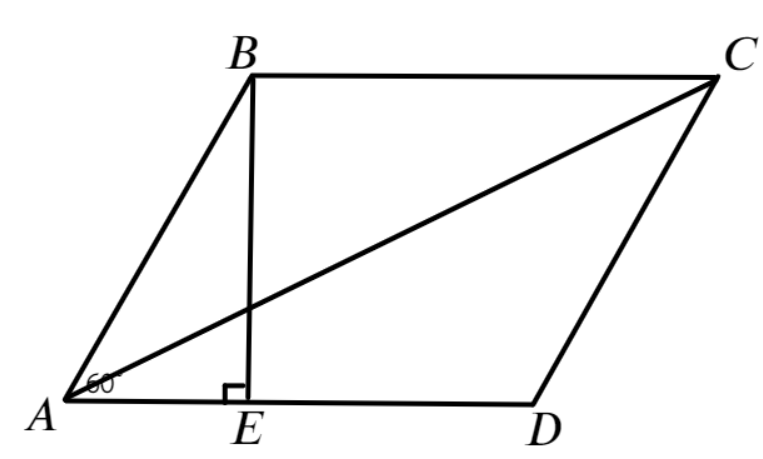
\includegraphics[scale=0.35]{g9-97.png}}
\end{figure}\\
Найдём $CD=AB=\cfrac{BE}{\sin(60^\circ)}=\cfrac{2\sqrt{3}}{\cfrac{\sqrt{3}}{2}}=4$ и $\angle D=180^\circ-60^\circ=120^\circ.$ Тогда по теореме косинусов получаем равенство $AC=\sqrt{4^2+2^2-2\cdot4\cdot2\cdot\left(-\cfrac{1}{2}
ight)}=2\sqrt{7}.$\\
